% vim: fileencoding=utf-8

\documentclass{beamer}

\usepackage[utf8]{inputenc}
\usepackage[russian]{babel}
\usepackage[T1]{fontenc}
\usepackage{graphicx}
\usepackage{listings} 
\usepackage{xcolor} 
\usepackage{amsmath}

\lstset{%
  language=Python,
  extendedchars={true},
  inputencoding={utf8},
  frame=leftline,
  % framexleftmargin=1cm,
  xleftmargin=0.5cm,
  numbers={left},
  numberstyle={\tiny},
  basicstyle={\ttfamily \scriptsize},
  keywordstyle={\rmfamily \bfseries},
  commentstyle={\rmfamily \itshape},
  tabsize={4},
  showstringspaces=false,
  breaklines=true,
  breakatwhitespace=true,
  escapechar=\%
} 

%% Preamble

\usetheme{Madrid}
\usecolortheme{whale}
% \setbeamersize{text margin left=1cm}

%% Title slide

\title[Вывод типов для Python в IDE]{ Вывод типов для языка Python в интегрированной среде разработки }
\author[М.В.~Голубев]{% 
  М.В.~Голубев 63501/13 \\ \vspace{.10cm} 
  {\small научный руководитель} \\ \vspace{.10cm} А.С.~Власовских, ст. разработчик, JetBrains
}

\institute[СПбГПУ]{
  % Институт информационных технологий и управления \\
  % Кафедра компьютерных систем и программных технологи
  \normalsize
  Направление: 230100 --- Информатика и вычислительная техника \\

  Магистерская программа: 230100.68.15 --- Технологии проектирования системного и
  прикладного программного обеспеченияй
}
\date[20.06.2014]{%
  \\ \vspace{1cm}
  \footnotesize Санкт-Петербургский государственный политехнический университет
}


%% Main content

\begin{document}

\frame{\titlepage}

\begin{frame}
  \frametitle{Проблема}

  В языках с динамической типизацией проверки типов осуществляются только во время исполнения программы.
  \begin{itemize}
      \item Примеры: Python, Ruby, Perl, JavaScript, Clojure и др.
      \item Достоинства:
        \begin{enumerate}
            \item Лаконичный синтаксис без аннотаций типов.
            \item Нет длительного этапа компиляции при разработке.
            \item Больше возможностей метапрограммирования.
        \end{enumerate}
      \item Недостатки:
        \begin{enumerate}
            \item Низкое быстродействие.
            \item \textbf{Нет встроенных средств для поиска ошибок типов.}
        \end{enumerate}
  \end{itemize}
    
\end{frame}


\begin{frame}[fragile]
  \frametitle{Пример ошибки типа}
  \framesubtitle{Обращение к несуществующему методу}

  \begin{lstlisting}[
    label={lst:type-error-sample},
    gobble={2},
  ]
  class MyClass(object):
    def method(self):
        print('Success')

  inst = MyClass()
  %\color{red}inst.missing()%

  %\color{red}getattr(inst, ''.join(['m', chr(105), 'ssing']))%()

  %\color{red}exec('inst' + '.missing()')%
  
  del MyClass.method
  %\color{red}inst.method()%

  \end{lstlisting}
    
\end{frame}

\begin{frame}
  \frametitle{Статический анализ}

  Решением является использование в процессе разработки инструментов,
  осуществляющих статический анализ программ для поиска ошибок.

  \begin{itemize}
      \item Пакетные анализаторы: PyLint, PyFlakes
      \item Среды разработки (IDE): \textbf{PyCharm}, PyDev, Wing IDE
  \end{itemize}
    
\end{frame}

\begin{frame}[fragile]
  \frametitle{Источники информации о типах}

  % \begin{lstlisting}[
    % label={lst:type-sources},
    % gobble=2
  % ]
  % def python_modules(dir_path:str, extension='.py'):
    % """Returns list of Python modules in directory.

    % :type extension: str
    % :type dir_path: str
    % :rtype: list[str]
    % """
    % assert isinstance(extension, str)

    % p = Path(dir_path)
    % result = []
    % for child in p.iterdir():
        % if child.is_file() and child.suffix == extension:
            % result.append(str(child))
    % return result
  % \end{lstlisting}
  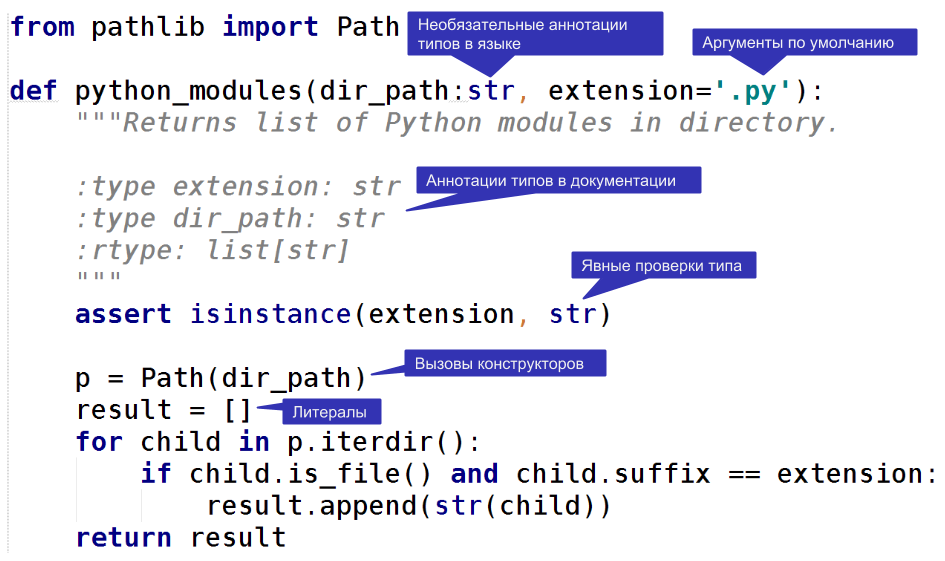
\includegraphics[width=0.9\paperwidth]{fig/type-sources-annotated.png}
    
\end{frame}

\begin{frame}
    \frametitle{Постановка задачи}
    \begin{block}{Задача}
        Разработать метод, при помощи которого можно было улучшить существующие
        возможности среды PyCharm по выводу типов в программах на Python.
    \end{block}

    Требования:
    \begin{itemize}
        \item Метод должен быть как можно более точным при, по возможности,
          наибольшей полноте.

        \item Метод должен иметь быстродействие, достаточное для его использования в
          IDE.

        \item Метод не должен нарушить работу имеющегося статического анализа в
          среде PyCharm.
    \end{itemize}
    
    \begin{block}{Выбранное направление}
      Вывод типов параметров функций.
    \end{block}

\end{frame}

\begin{frame}[fragile]
  \frametitle{Предлагаемый подход}
  
  Пример:
  \begin{lstlisting}[
    label={lst:uninferred-types},
    gobble=2
  ]
  def sanitize_url(url):
      sanitized = url.lower()
      if url.endswith('/'):
          sanitized = sanitized[:-1]
      return sanitized
  \end{lstlisting}
  
 Предполагаемый тип функции: $str \rightarrow str$. Сейчас PyCharm не может
 вывести ее тип.

 \begin{block}{Основная идея}
   Подбирать возможные классы для параметров функций на основе информации об
   используемых атрибутах объекта. 
 \end{block}
    
\end{frame}

\begin{frame}[fragile]
  \frametitle{Предлагаемый подход}
  \framesubtitle{Продолжение}
  
  Пример:
  \begin{lstlisting}[
    label={lst:uninferred-types},
    emph={lower,endswith},
    emphstyle=\color{blue},
    gobble=2
  ]
  def sanitize_url(url):
      sanitized = url.lower()
      if url.endswith('/'):
          sanitized = sanitized[:-1]
      return sanitized
  \end{lstlisting}

  \begin{itemize}
      \item Свяжем с параметром  \texttt{url} \emph{структурный тип}: $\{ lower,
        upper \}$ и найдем все известные классы (\emph{номинальные типы}),
        совместимые с данным структурным. Например, \texttt{str | bytearray | bytes}.

      \item Ранее подобный подход был описан для языка Smalltalk в работе F.
        Pluquet, A.  Marot, R. Wuyts ``Fast type reconstruction for dynamically
        typed programming languages''.

      \item Главную сложность представляет наследование.
  \end{itemize}
  


\end{frame}

\begin{frame}
  \frametitle{Поиск унаследованных атрибутов}
  \framesubtitle{Подход, предложенный в публицкации}
    
  Ищем наиболее общий класс с атрибутами \texttt{m1} и \texttt{m2}, спускаясь от
  корня в дереве наследования классов.

  \begin{figure}
    \begin{center}
      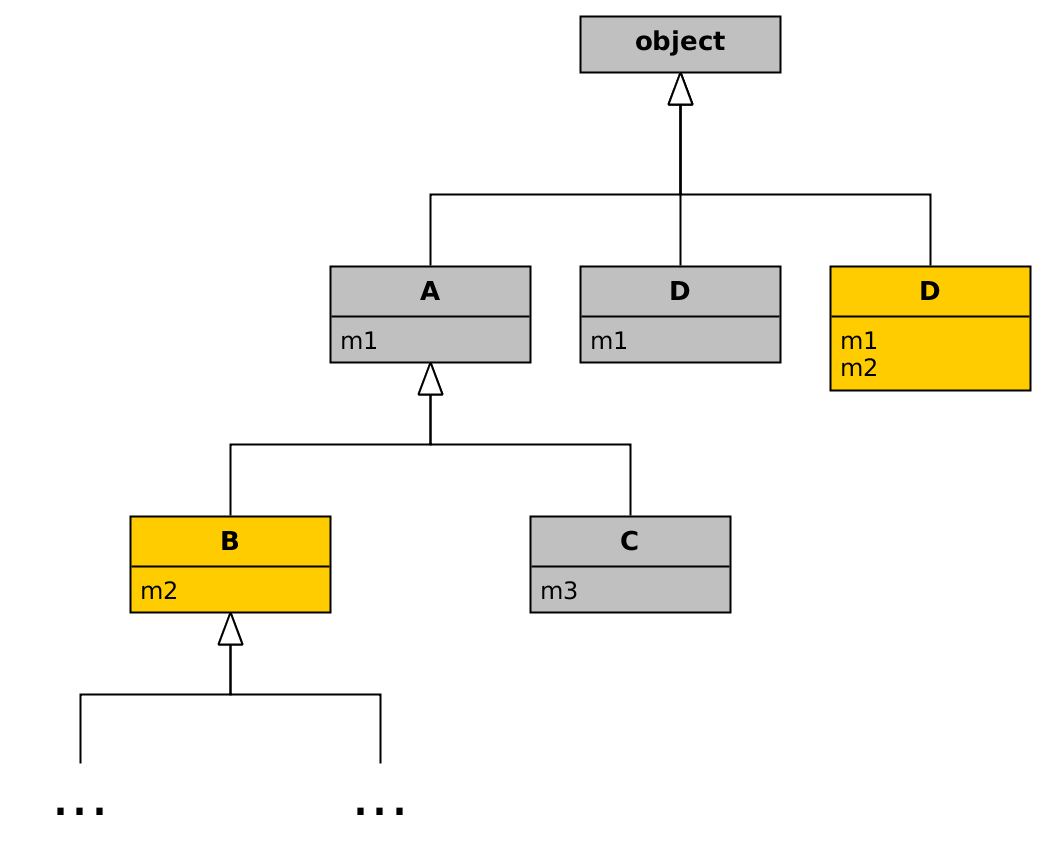
\includegraphics[width=0.6\linewidth]{fig/class-search-example.png}
    \end{center}
  \end{figure}
\end{frame}

\begin{frame}
  \frametitle{Поиск унаследованных атрибутов}
  \framesubtitle{Ограничения описанного подхода}

  Такой подход неприменим в PyCharm:
  \begin{itemize}
      \item В Python возможно множественное наследование между классами.

      \item Такая иерархия не хранится в памяти целиком: быстрый поиск классов
        осуществляется при помощи индексов. Поддерживать подобное дерево с
        учетом постоянно изменяемых исходных текстов проекта было бы чрезвычайно
        трудоемко.
  \end{itemize}
  
\end{frame}

\begin{frame}
  \frametitle{Поиск унаследованных атрибутов}
  \framesubtitle{Использование индексов для поиска классов}
  
  Индекс --- плоская база данных типа ключ-значение.

  Идеальный вариант --- построить индекс $ClassesWithAttributes^*$ вида

  \begin{multline*}
    AttributeName \rightarrow \{class: AttributeName \in \\
  (DeclaredAttributes(class) \cup InheritedAttributes(class)) \}
  \end{multline*}

  Тогда поиск подходящих классов для параметра $p$ сводится к операции

  \[
    suitableClasses_p = \bigcap\limits_{\forall{a} \in AccessedAttributes(p)}
    ClassesWithAttribute^*(a)
  \]
  
\end{frame}

\begin{frame}
  \frametitle{Поиск унаследованных атрибутов}
  \framesubtitle{Использование индексов для поиска классов (продолжение)}

  Использование индекса $ClassesWithAttribute^*$ нарушает свойство
  \emph{инкрементальности}, или модульности анализа.

  \begin{block}{Свойство инкрементальности}
    Инкрементальный анализ не требует переиндексации каких-либо модулей
    кроме текущего.
  \end{block}

  В индексе $ClassesWithAttribute^*$ изменение какого-либо базового класса
  потребует изменения записей индексов для всех его наследников.
\end{frame}

\begin{frame}
  \frametitle{Поиск унаследованных атрибутов}
  \framesubtitle{Предлагаемое решение}

  Строим более простой индекс $ClassesWithAttribute$
  \begin{multline*}
    AttributeName \rightarrow \{class: AttributeName \in DeclaredAttributes(class) \}
  \end{multline*}

  На первом шаге алгоритма делаем предвыборку всех классов-кандидатов для
  параметра $p$:  
  \[
    candidateClasses_p = \bigcup\limits_{\forall{a} \in AccessedAttributes(p)}
    ClassesWithAttribute(a)
  \]

  Далее ищем унаследованные атрибуты, исключая из множества неподходящие классы.
    
\end{frame}

\end{document}
